%%%%%%%%%%%%%%%%%%%%%%%%%%%%%%%%%%%%%%%%%%%%%%%%%%%%%%%%%%%%%%%%%%%%%%%%%%%%%%%%
\section{Understanding Typos Empirically}
\label{sec:mturk}
\def\shift{\ensuremath{\langle s \rangle}}
\def\caps{\ensuremath{\langle c \rangle}}
\newcommand{\plotmturk}[8]{{
    \begin{tikzpicture}[scale=0.55]
      \begin{axis}[
        axis y line*=left,
        ymin=0, ymax=50,
        #3,
        % xlabel={\large #3},
        % ylabel={\large #5},
        y axis style=black!50!black,
        xtick=data,
        xticklabels from table={#1}{#2},
        legend style={at={(0.97,0.97)}, anchor=north east},
        ybar
        ]
        \addplot[color=blue!50] table [x={index}, y={#4}]  #1;
        \legend{#7}
      \end{axis}

      \begin{axis}[
        ymin=0.03, ymax=0.10,
        axis y line=right, 
        axis x line=none,
        xticklabels={},
        y axis style=red!90!red,
        #5,
        legend style={at={(0.97,0.88)}, anchor=north east},
        y tick label style={/pgf/number format/fixed,
          /pgf/number format/1000 sep = \thinspace % Optional if you want to replace comma as the 1000 separator 
        }
        % scaled y ticks={base 10:2}
        ]
        \addplot [sharp plot, color=red!90, mark=*] table [x={index}, y expr=\thisrow{#6}/100.00] #1;
        \legend{#8}
      \end{axis}
    \end{tikzpicture}
  }}




%%%%%%%Average typing speed of the worker and probability of making typo%%%%%%%
%%%%%%%%%%% Typist speed and Typo %%%%%%%%%%%%%%%
%  index,speed(cpm),totalsample(%),typo(\%)
%   0,133.00,21.28,6.69
%   1,181.90,23.58,5.60
%   2,219.55,25.66,5.30
%   3,299.26,29.49,4.96
%%%  Average of the average typing speeds for the 
%%%  workers in that group
%%%%%%%%%%%%%%%%%%%%%%%%%%%%%%%%%%%%%%%%%%%%%%%%%%

\pgfplotstableread[col sep=comma, format=inline] {
index,typingtime,totalsample,typo
0,1.18,25,3.66
1,2.01,25,4.84
2,3.07,25,5.88
3,6.89,25,7.88
}\typingtimetypo

%%%%%%%%%%%%%%%%%%%%%%%%%%%%%%%%%%%%%%%%%%%%%%%%%%%%%%%%%%%%%%%%%%%%%%%%%%%%%%%%
%%%%%%%%%%%Time to type a pw and typo %%%%%%%%%%%%
% index,typingtime(sec),totalsample(%),typo(%)
% 0,1.18,25.00,3.66
% 1,2.01,25.00,4.84
% 2,3.07,25.00,5.88
% 3,6.89,25.00,7.88
%%% The typing time is the average typing time for
%%% the passwords in that group
%%%%%%%%%%%%%%%%%%%%%%%%%%%%%%%%%%%%%%%%%%%%%%%%%%

%% Old data
% \pgfplotstableread[col sep=comma, format=inline] {
% index,tspeed,totalsample,typo
% 0,133,21.28,6.69
% 1,182,23.58,5.60
% 2,220,25.66,5.30
% 3,299,29.49,4.96
% }\tspeedtable

%% New data
\pgfplotstableread[col sep=comma, format=inline] {
index,tspeed,totalsample,typo
0,109,21.9,6.4
1,150,23.3,5.6
2,182,25.4,5.2
3,245,29.4,5.2
}\tspeedtable

%%%%%%%%%%%%%%%%%%%%%%%%%%%%%%%%%%%%%%%%%%%%%%%%%%%%%%%%%%%%%%%%%%%%%%%%%%%%%%%%
%% Passsword length and typo
\pgfplotstableread[col sep=comma, format=inline] {
 index,length,totalsample,typo
0,$<5$, 17.9, 7.69
1,6--7, 20.5, 9.44
2,8--9, 20.5, 10.0
3,10--11, 20.5, 11.02
4,12--25, 20.51,13.28
}\lengthtypotable

%% Old data
 % 0,$\le5$,3.6,4.6
 % 1,6--7,41.1,5.0
 % 2,8--9,33.9,5.9
 % 3,10--11,14.6,6.6
 % 4,$\ge12$,6.9,9.2



%%% Password length for 5,000 passwords
% \pgfplotstableread[col sep=comma, format=inline] {
%  index,length,totalsample,typo
%  0,$\le 5$,17.9,3.8
%  1,6--7,20.51,4.42
%  2,8--9,20.51,6.12
%  3,10--11,20.51,6.68
%  4,$\ge12$,20.51,10.16
% }\lengthtypotable

%%%%%%%%%%%%%%%%%%%%%%%%%%%%%%%%%%%%%%%%%%%%%%%%%%%%%%%%%%%%%%%%%%%%%%%%%%%%%%%%
%% Password complexity and typo
\pgfplotstableread[col sep=comma, format=inline] {
  index,cmplcl,totalsample,typo
  1,1,23.88,4.72
  2,2,25.42,6.59
  3,3,25.38,10.19
  4,4,25.32,14.91
}\complexitytypotable



%%%%%%%%%%%%%%%%%%%%%%%%%%%%%%%%%%%%%%%%%%%%%%%%%%%%%%%%%%%%%%%%%%%%%%%%%%%%%%%%
%% Password popularity and typo
\pgfplotstableread[col sep=comma, format=inline] {
  index,freqrange,totalsample,typo
  3,$1$,36.3,5.42
  2,2--11,21.4,4.09
  1,12--211,21.1,3.52
  0,$f>211$,21.1,2.68
}\populartypotable








% %%%%%%%%%%%%%%%%%%Typing time and typo%%%%%%%%%%%%%%%%%%%%%%%%%%%%%%%%%%%%%%%%%%
% \begin{figure}[t]
%   \centering
%   \plotmturk{\typingtimetypo}{typingtime}{Time required to type (sec)}{totalsample}{Total number of sample (\%)}{typoa}{Percentage of typos (\%)}
%   \caption{Probability of a password being mistyped is positively
%     correlated with the amount of time spent in typing the
%     password. We split the passwords into four quartiles based
%     on the amount time spent by workers to type them, and then compute
%     the fraction of passwords mistyed for each quartile. X-axis labels
%     are average time spent on typing a password in corresponding
%     quartile.}
%   \label{fig:typetime-typo} 
% \end{figure}

% %%%%%%%%%%%%%%%%%%Length of a password and typo %%%%%%%%%%%%%%%%%%%%%%%%%%%%%%%%%%%%
% \begin{figure}[t]
%   \centering
%   \plotmturk{\lengthtypotable}{length}{Length of passwords}{totalsample}{Total number of samples (\%)}{typo}{Percentage of typos (\%)}
%   \caption{The fraction of mistyped passwords broken down by password length
%     ranges.} 
%   \label{fig:length-typo}
% \end{figure}




%%% Local Variables:
%%% mode: latex
%%% TeX-master: "main"
%%% End:



We start with experiments using Amazon Mechanical Turk (MTurk) ~\cite{buhrmester2011amazon} to
measure the kinds of typos that people make when typing passwords.
The goal of this preliminary measurement study is to discover the most
frequent typos across a population for typical user-chosen
passwords. We will follow on up these MTurk experiments with real user
data using instrumentation of the Dropbox operational environment
(discussed in \secref{sec:dropbox}).

\paragraph{Experiment design.} 
% \devd{didn't know where to put this note, but we compare to Dropbox data later,
% but the MTurk data is not limited to length 6 or more, is it? Can we remove all
% the less than 6 chars case for the comparison?}
MTurk allows custom-designed human-intelligence tasks (HITs) to be
submitted to workers over the
web. %Our experimental design revolves around a
We created a password-typing HIT that asks a worker to type $k$
passwords within a given time limit. Inside a HIT, every password
needs to be typed within a conventional HTML password-type input box,
i.e., each typed character shows up as a dot. Copy-paste functionality
is disabled in the input boxes using the html ``{\tt onpaste=false
  oncopy=false}'' option. This check can be circumvented by changing
the browser settings, but we recorded all key presses inside an input
box and used this to help filter out copy-paste attempts. We did not
find any circumvention in the collected data.

Our MTurk experiment design mainly aims at gathering data efficiently to
identify common typos and trends. We note that the typos found in transcribing
passwords in MTurk may not be truly representative of the typos users make when
typing their own passwords. Performing a longitudinal study using MTurk where
users retype their chosen password multiple times would be interesting, but it
would be logistically complicated and would greatly slow the data collection
rates while still not providing real ecological validity~\cite{fahl2013ecological}. The reasons for
experimenting in MTurk is that prospecting for common typos in a real
operational environment, such as Dropbox's, would seem to require 
storing information about plaintext passwords in between logins, which could
represent a significant security problem.
%engineered sites such as Dropbox do not store users' passwords explicitly.  
Thus we adopt the two-phase investigative approach. First prospecting for common
typos via MTurk and, given a list of such typos, presenting a measurement
of real-world Dropbox user typos later in the paper.

% In two-third of the HITs we displayed
% indicators to to notify the user whether or not the caps lock key is
% pressed, remaining one-thrid of the HITs do not have any indicator. We
% used two types of caps lock indicators used in equal number of HITs;
% the first one is a very faint warning symbol displayed below the input
% box whenever the caps lock key is active; the second type of indicator
% is bold red color text written "Caps Lock" will appear whenever the
% caps lock key is active. (See~\figref{fig:hit} for details.)



% We additionally perform experiments of the same form while requesting
% the workers to complete the task using devices having touchscreen
% keyboards.  An increasing fraction of password logins occur via
% smartphones, ipads and tablets which only have touchscreen keyboards,
% and typing on these devices is significantly different from typing on
% general keyboards. We change the HIT to check the device from which
% the page is accessed (as reported via the browser's user agent
% string).  Here we decrease the number of passwords to type in an HIT
% compared to the non-targeted case above.

%We begin with a set of
%transcription experiments in which we task workers with typing in
%passwords shown to them.  
In our MTurk experiments we ask workers to type the passwords which are
sourced from the RockYou password leak~\cite{rockyou:2009}.  This data
set is the largest plaintext password leak to date, with passwords
from over 32 million users.  It has been used widely for 
password-related studies and the distribution of passwords is similar to other
leaks.  The data set contains a number of passwords that may be
objectionable to some people (e.g., many popular passwords are based
on profanities from a wide number of languages). Instead of removing
these passwords, which would bias the study, we used the MTurk
mechanism of indicating that there may be vulgar content in the
HITs. This restricts the HITs to be used only by adult workers as well
as providing a warning to them about the potential for objectionable
content. We also removed all passwords of length greater than 25, as
these are (by manual inspection) not user-selected passwords.

Amazon allows the HIT creator to specify the required qualification
and location of the worker. We allowed workers with more than 10\%
acceptance rate\footnote{Acceptance rate in MTurk paradigm
  means the percentage of HITs, that the worker has submitted, have been
  accepted by the requester of the work. This is an eligibility filter
  provided by MTurk. } and that were located in countries whose official
language is English.  % \fixme{What does 10\% acceptance rate mean?}
%The latter matches the fact that
% the passwords were sourced from an English-language site.

None of the data we recorded contains personally identifying information. We
nevertheless submitted our experiment designs to our institutional review board
and received an IRB exemption.

%Studies have shown long passwords and passwords with s% acceptance rate mean?}ymbols, digits and mixed
%cases are more prone to mistakes~\cite{mazurek:2013:mpg, shay:2010:encounter}.

\subsection{Measured Typo Rates}

%We start by considering RockYou restricted to passwords of length 6 or more. The
%length requirement matches the Dropbox policy for passwords (see the next section). 
We sampled 100,000 passwords randomly with replacement
according to the empirical probability distribution of RockYou passwords of
length 6 or more.  (The
length requirement matches the Dropbox policy for passwords, as discussed in the
next section.) By sampling
with replacement, this means we match the expected distribution of
submitted passwords a web service might see across their entire user base 
(e.g., the password
``123456'' appears frequently).  We split the sample into HITs,
ensuring that none of the HITs contain more than 180 characters in
total. (This approximately normalizes the amount of typing effort of a
single HIT.)  %An example of a HIT is shown in \apref{sec:hit}. 
Each
MTurk worker is given 300 seconds to type all the passwords in the
HIT. The number of passwords in a HIT ranges between 16 to 22.  To
ensure a broad pool of users, a worker is only allowed to submit a
maximum of 3 HITs. To impose this restriction, we used a third-party
JavaScript function provided by a website called Unique
Turker~\cite{uniqturker}.  In addition to the submitted passwords, we
collected the user agent string of the browser from which the worker
submitted the job, and all the key presses (and their timestamps)
inside the input boxes within the HIT.


%\paragraph{Gathered data.} 
A total of 4,362 workers participated in our study. Several passwords
were not typed at all (e.g., the worker accidentally submitted the HIT
before typing all the passwords), and sometimes the wrong password was
entered (e.g., when prompted ``123456'' the user entered
``password'').  % We resubmitted these passwords by creating new
% HITs. \fixme{why?}  After the re-submission, 

\paragraph{Sanitization.} We sanitize the received data first, by removing
the submissions where either no password was typed or typed passwords have a
case-independent edit distance of five or more from the prompted password.
 This excluded 226 of the password samples.  Here and
throughout this section edit distance includes insertions, deletions, and
substitutions each as unit cost. 


Preliminary analysis of the remaining data revealed that a large
fraction of errors were caused by accidental pressing of the caps-lock
key. Looking at the data, it was clear that in many cases workers had caps lock
on for a large number of contiguous entries.  We therefore sanitized our data 
with a heuristic to figure out improper propagation of caps-lock errors across
multiple entries.
The details are given in \apref{app:caps-lock-err}.


%There were in total 81,595 unique passwords in this set of submissions.  
After sanitization, there were in total 4,364 incorrect submissions
across 97,632 valid submissions (4.5\%).  There were 81,595 unique
passwords among the sanitized submissions, and 5.5\% of all unique
passwords were mistyped at least once.  Because we instrumented all
key presses, we could see when users corrected entries before
submission. An additional 8.2\% of submissions were first incorrectly
typed by the workers, but corrected before submission.  In total, we
found that 42\% of the workers made at least one typo across all their
submissions, while 1.6\% submitted more than four mistyped passwords
in their submissions.

%Across
% all submissions (including
%repeats of passwords), 14.7\% were typed incorrectly  
%in a first attempt.  the majority of incorrectly typed passwords (62\%) %9.1\% 
%were corrected by the worker before
%being submitted. The remaining 38\% were submitted and in total this gives 5,554
%submitted incorrectly typed passwords (5.6\% of all typed passwords).

From now on our analyses are based on the submitted passwords unless otherwise
specified. We include duplicate passwords in our analyses because they reflect
the distribution of passwords a provider would see.  


The data resulting from the MTurk measurements suggest that there is some correlation
between typo likelihood and password complexity under various measures such as length and lexical
diversity.  As this is not our main focus we defer discussion to
\apref{app:complexity}. 
%It is possible that the passwords from the more complex buckets
%are also longer in size. We therefore also report the percentage
%of typos for each of the length groups as we defined above. \tnote{I don't
%understand this}
%We warn that there aren't many passwords for all length 
%groups for each complexity bucket.\tnote{need to probably revisit this and
%figure out what can be said more specifically}



%%%%%%%%%%%%%%%%%%%%%%%%%%%%%%%%%%%%%%%%
\subsection{The Nature of Typos} 
%%%%%%%%%%%%%%%%%%%%%%%%%%%%%%%%%%%%%%%%
%\subsection{Analysis of Typo Types}

We now analyze the nature of typos made by the MTurk workers.  First, we look at
typos based on the \edistname between the mistyped password and the correct
password. For 86\% of incorrectly typed passwords, if we normalize the cases of
alphabetic characters, the \edistname between the submission and the correct
password was one.  This suggests most password typos are relatively simple.

To obtain better clarity on the kinds of typos made, we analyze 
typographical errors on a representation of strings 
that accounts for the keys that must be pressed while entering it. 
This allows us in particular to highlight the role of
capitalization errors due to shift and caps-lock mistakes during password entry. 

The key-press representation of a string is defined as follows. First, recall
that our standard alphabet includes 
upper- and lower-case letters, numbers, symbols, and
the space character. We define a key-press alphabet that includes only the keys
on a standard US keyboard: lower-case letters, numbers, symbols that can be
entered without shift (such as the period), the caps-lock key denoted
by $\caps$, and either shift key represented by $\shift$. 
%These new characters represent, respectively,
%pressing the caps lock key and holding down either shift key while pressing the
%next character.  
Then, we convert each password and submitted string from the MTurk
study to a key-press string by replacing characters omitted from the
key-press alphabet by appropriate combinations of $\shift$ or $\caps$ tokens
and tokens for keys in the key-press alphabet.  We heuristically assume any sequence
of 3 or more capital letters was entered using caps lock and
singleton or doubles using a shift key.  So for example, the string
``{Password}'' would be converted to the string
``{$\shift$-p-a-s-s-w-o-r-d}'' over our new alphabet, and likewise
``{ABC12!@}'' would be converted to
``{$\caps$-a-b-c-$\caps$-1-2-3-$\shift$-1-$\shift$-2}''.  As seen in
this last example, in our conversion we insert a $\shift$ token for each
character modified by it (despite the fact that the user may hold it
down for the duration).
%
%For simplicity, we assumed that shift key is pressed every
%time it needs to be activated.  The algorithm to convert an arbitrary
%string to the corresponding key-press sequence is given in
%\apref{ap:keypress-sequence}.  
%We assumed US keyboard layout for
%converting the strings to the sequence of key-presses.  \footnote{This
%  assumption might not be valid, but helps keeping the analysis simple
%  and clear.\fixme{the last sentence}}. For example, ``{Password}''
%will be converted to ``{$\shift$-p-a-s-s-w-o-r-d}'', and ``{ABC12!@}''
%will be converted to
%``{$\caps$-a-b-c-$\caps$-1-2-3-$\shift$-1-$\shift$-2}''.  
%For the rest
%of this subsection, a string is in the key-press representation.

To gain insight into what kinds of typos the workers made, we constructed a confusion matrix
in which rows represent the true keys that should have been pressed, and
columns represent the keys that were actually pressed.  We filled this matrix
in the following way. For each pair of prompted password and
submitted string, we find an optimal alignment of the corresponding
key presses that minimizes the total cost of the edit operations.  We
can extract an optimal alignment in the process of computing the
minimum edit distance using a dynamic programming algorithm approach proposed
in~\cite{smith1981identification}.  We then counted the frequency of
$c\rightarrow c'$ pairs, where $c$ is the key in the given password
and $c'$ is the key which is typed. We allowed $c$ to take on a placeholder value
[ins] signifying when $c'$ was inserted into a password, and $c'$ to
take on a placeholder value [del] to denote that $c$ was deleted from
a password. We omitted the case $c = c'$ from our tabulation, as it represents no typographical error.

For example, consider if the prompted password was the string ``Password'', (or
``{$\shift$-p-a-s-s-w-o-r-d}'' in key-press representation) and the study
participant submitted the string ``passw0rd1'' (or ``{p-a-s-s-w-0-r-d-1}'' in
key-press representation). Our algorithm would increment the counts for
$\shift \rightarrow \textnormal{[del]}$, $o \rightarrow 0$, and
$\textnormal{[ins]}\rightarrow 1$. The corresponding typos are: forgetting $\shift$ to
capitalize the first letter, changing an `o' to `0', and adding a (spurious) `1' at the end. 

The histogram resulting from doing this for all submitted passwords is shown as
a heatmap in \figref{fig:heatmap}. Darker colors signify
higher counts.  The keys are sorted according to a standard 
US keyboard layout.



\begin{figure}[t]
  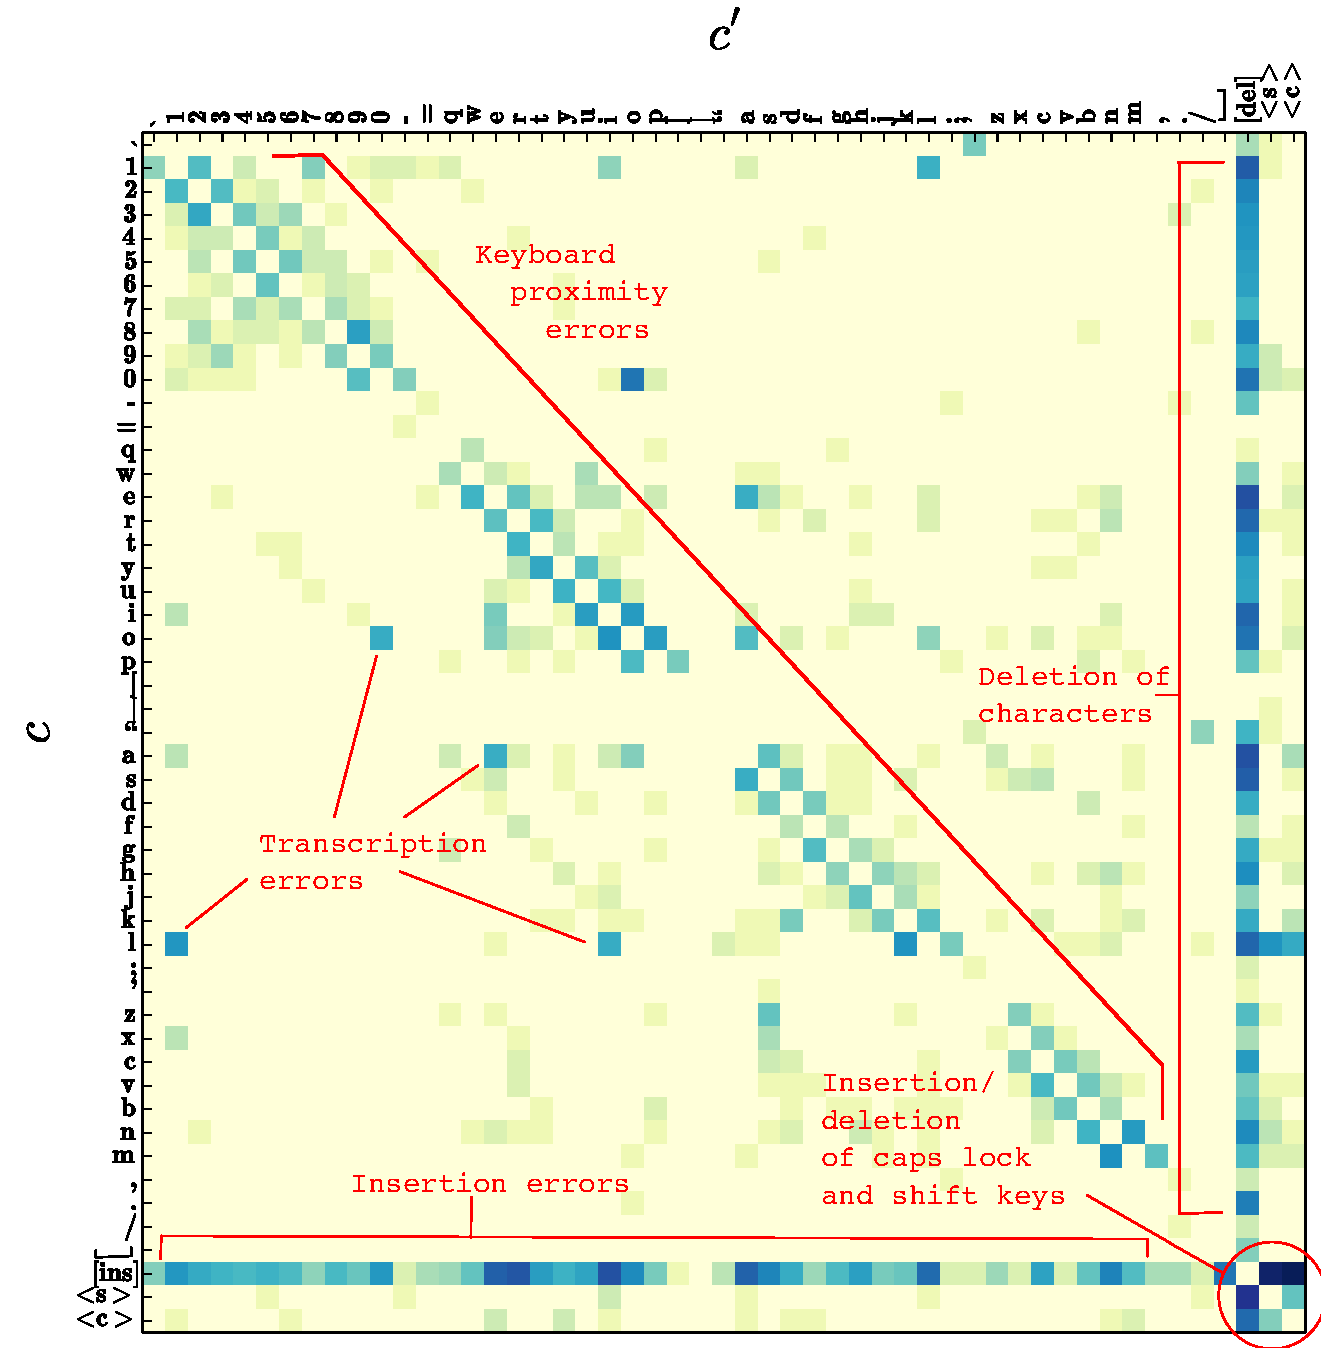
\includegraphics[height=0.48\textwidth]{images/heatmap}
  \caption{Heatmap showing the counts of edits that arose in computing
    \edistname from the key-press sequence of the submitted passwords
    to the key-press sequence of the prompted passwords. The color in
    row $c$ and column $c'$ indicates how often the edit
    $c \rightarrow c'$ was observed across all distance
    calculations. The darker the color the higher the count.  Labels
    [ins] and [del] denote insertion (character mistakenly inserted)
    and deletion (failure to type a character). Tokens \textvisiblespace $\,$, $\shift$, and $\caps$
respectively denote the and space-bar, shift, and caps lock.}
  \label{fig:heatmap}
\end{figure}


Several common typographical errors stand out:
\begin{newitemize} 
\item \emph{Insertion and deletion of shift and caps-lock keys}: In the right
  bottom corner appears a dark patch of $3\times3$ squares. This reflects the
  frequency of erroneous use or lack of use of shift and caps
  lock---equivalently, incorrect insertion or deletion of the $\shift$ and
  $\caps$ tokens.  These typos will switch the case of the password if it
  contains English letters as well as changing the shift status of digits and
  symbols (e.g., $4\rightarrow \$$).
  % (last two columns of the row $c=\mbox{[ins]}$) and deleted (last two
  % rows for the column $c=\mbox{[del]}$). 

%\item \emph{Number/symbol errors}: The diagonal in the symbol rows starting with
%$c = \textrm{@}$  reveal shifting errors in which symbols were accidentally typed as
%numbers. There is a symmetric diagonal showing numbers being mistakenly typed as
%symbols. 
%
\item\emph{Keyboard proximity errors}: The slightly darker cells near
  the diagonal represent typos due to mistakenly pressing a
  neighboring key to the left or right of the intended key.  
  We found more generally that there are a significant number of typos for which a key is
replaced by an adjacent one (left, right, above, or below).
  We collectively refer to these as proximity errors.

\item \emph{Number-to-number errors}: We see a
  square cluster of moderately high-frequency errors in the top left that represent digit-to-digit typos. Some of these are
  proximity errors, but many such errors confuse
  widely separated numbers, e.g., $3\rightarrow 9$.
  
%The bulk password characters are lower-case letters. \tnote{need more analysis --- nearby
%characters?}
\item \emph{Insertions and deletions}: There are throughout a large
  number of insertion (third row from the bottom) and deletion (third
  column from the right) errors. Deletions are slightly more common.
  %
\item\emph{Transcription errors}: The heatmap has sporadic dark cells, including
  \mbox{(l,1), (o,0), (0,o), (l,i)}. These represent transcription
  errors due to a worker confusing similar-looking characters. We presume that 
  the prevalence of reading errors are an artifact of the experiment design, and will be less frequent for entry of memorized passwords.
  Nevertheless, such errors could arise for users that write down 
  their passwords to remember them.
 % The worker got confused between to very similar looking
 % characters such as l (ell) and 1 (one).
\end{newitemize}
Our analysis suggests that a large fraction of common typos fall into a few
classes. A subset of these are what we refer to as ``easily correctable,'' as we
discuss shortly.

\subsection{Touchscreen Keyboards}
We performed a smaller, but similar, study in which workers were
required to use touchscreen keyboards. The hypothesis here is that the
distribution of typos may differ due to keyboard type. We submitted
24,000 passwords drawn from RockYou across 1,987 HITs using the same
methodology of approximately normalizing effort by restricting total
character counts to be less than 110.  Workers were given 300 seconds
to perform a HIT. We restricted workers to using touchscreen keyboards
by checking the {\tt user-agent} string of the worker's browser.

Unlike the desktop user experiment earlier in this section, we did not need to
adjust for the caps lock propagation error on touchscreen devices. This was
because of the fact that in touch screen devices the caps lock key is auto reset
every time the focus shifts from one input field to the other. We performed an
analysis that was otherwise similar to the analysis used above for the general
MTurk experiment. To calculate proximity errors, we used the Android keyboard
layout, which we believe is a sufficiently good proxy for all touch screen
keyboards.  

The probability of a typo here was 9.0\%, an increase over the 4.5\%
for unrestricted workers.  We compare the types of typos across the
two data sets quantitatively below.
 

\subsection{Easily-Correctable Typo Classes and Correctors}

Using all the data above we manually enumerate a set of common typo
types, or classes.  The resulting classes are detailed in
\figref{fig:top10-typo}, and shown for both the first general MTurk
experiment and the touchscreen-restricted experiment.  The column
labeled ``Corrector'' identifies the function that can be used to
correct the corresponding typos: $\swcall$ switches the case of all
letters in a password, $\swcfirst$ switches the case of the first
letter, $\rmlast$ removes the last character, $\rmfirst$ removes the
first character, and $\dtoslast$ changes the last character to its
equivalent character under the shift-key modifier (e.g., `1' becomes
`!', `a' becomes `A', etc.). The correctors mentioned above are
mutually exclusive, that is, any two correctors, when applied to an
input password of length larger than one, will produce two different
passwords (assuming at least one of the correctors is applicable).


\begin{figure}[t]
  \centering
  \small
  \begin{tabular}[t]{p{1.55in}lrr}
    \toprule
    \multirow{2}{*}{\textbf{Typo type}}     & \multirow{2}{*}{\textbf{Corrector}} & \multicolumn{2}{c}{\textbf{\% of typos}}\\\cline{3-4}
    &&\multicolumn{1}{c}{\textbf{Any\Tstrut}} &
    \multicolumn{1}{c}{\textbf{Mobile}} \\\midrule
    Case of all letters flipped & \swcall & 10.9 & 8.3\\
%    \midrule
    Case of first letter flipped & \swcfirst & 4.5 & 4.7\\
%    \midrule
    Added extra character to end & \rmlast & 4.6 & 0.9\\
%    \midrule
    Added extra character to front & \rmfirst & 1.3 & 0.5\\
%    \midrule
    Missed shift for symbol at end  &  \dtoslast & 0.2 & 0.1\\
    % \midrule
%    \midrule
    Proximity errors & n/a & 21.8  & 29.6\\
    %Character replaced w/ nearby character on US keyboard 
%    \midrule
    Transcription errors & n/a& 3.0 & 3.3\\
%    \midrule
    Other errors & n/a & 53.6 & 52.7\\ 
    % Upper case to Title case and vice verse  &  \upncap & 0.2 & 0.3\%\\
    % \rownumber. & \stodlast & Last character symbol-to-number & 1\%\\
    % Change the shift state of the last non-letter character & \swslast& 0.3\%\\
    \bottomrule
  \end{tabular}

%   \begin{tabular}[t]{p{2.0in}lrrr}
%     \toprule
%     \multirow{2}{*}{\textbf{Typo type}}     & \multirow{2}{*}{\textbf{Corrector}} & \multicolumn{3}{c}{\textbf{\% of typos}}\\\cline{3-5}
%     &&{\bf general} & \pbox{1in}{\bf general\\(adjusted)} & \pbox{.8in}{\bf touchscreen \\device} \\\midrule
%     Case of all letters flipped & \swcall & 30.9\% & 10.9\% & 8.3\%\\
% %    \midrule
%     Case of first character flipped & \swcfirst &3.8\% & 4.5\% & 4.8\%\\
% %    \midrule
%     Added extra character at the end & \rmlast &3.5\% & 4.6\% & 6.6\%\\
% %    \midrule
%     Added extra character at the front & \rmfirst &  1.3\% & 1.3\% & 1.1\%\\
% %    \midrule
%     Missed shift key for the last symbol &  \dtoslast & 0.2\% & 0.2\% & 0.0\%\\
%     % \midrule
% %    \midrule
%     Proximity errors & n/a & 17.3\% & 21.8\%  & 29.6\%\\
%     %Character replaced w/ nearby character on US keyboard 
% %    \midrule
%     Transcription errors & n/a & 2.3\% & 2.99\% & 3.4\%\\
% %    \midrule
%     Other errors & n/a & 41.0\% & 53.6\% & 45.7\%\\ 
%     % Upper case to Title case and vice verse  &  \upncap & 0.2 & 0.3\%\\
%     % \rownumber. & \stodlast & Last character symbol-to-number & 1\%\\
%     % Change the shift state of the last non-letter character & \swslast& 0.3\%\\
%     \bottomrule
%   \end{tabular}
  
  \caption{The top categories of typos observed in our MTurk experiments.  The
    ``Corrector'' column identifies an (easily applied) function that corrects
    the typo. The ``Any'' column is percentage of typos by category for the
    initial MTurk study in which workers could have used any browser. Of 97,632
    passwords drawn from RockYou, 4,364 were mistyped.  The ``Mobile'' column is
    the same for the 23,098 submitted passwords collected from devices with
    mobile browsers.  Of these, 2,075 had a typo. }
\label{fig:top10-typo}
\label{fig:top-typo-mobile}
\end{figure}



As can be seen, the distribution of typos is non-uniform. A few typo classes
account for a large proportion of mistakes made. Caps-lock errors alone
represent 9.2\% of all mistakes made in our general MTurk experiments, and
proximity errors for another 21.8\% of all mistakes.
For mobile, we see a proportionally larger number of keyboard
proximity typos.


If a class of typo has a uniquely determined associated corrector, we refer to
it as {\em easily correctable}. The typo that produces a flipped case in the
first letter is an example: The corresponding corrector just flips the case of
the first letter. Not all easily correctable typos have involutory correctors
(the typo and corrector are the same function): consider the case of adding a
character to the end of a password which is corrected by removing a character. 

In contrast to easily correctable typos, a proximity error is hard to correct.
Given a password with a proximity error, correction would require
identification of the erroneous character as well as identification of the
nearby character that was the original, true one. Thus the space of possible
correctors for a proximity error is generally large. As we shall see later,
both security and performance are adversely impacted by searching large spaces
of correctors.


Our exploration culminates in the following two key results: {\em (1) Some typos
are significantly more common than others} and {\em (2) Many common typos are
easily correctable}. In the next section, we report on experiments at Dropbox
that verify that common, easily correctable typos arise frequently in practice.




%%%%%%%%%%%%%%%%%%%%%%%%%%%%%%%%%%%%%%%%%%%%%%%%%%%%%%%%%%%%%%%%%%%%%%%%%%%%%%%%
% JUNKYARD
%%%%%%%%%%%%%%%%%%%%%%%%%%%%%%%%%%%%%%%%%%%%%%%%%%%%%%%%%%%%%%%%%%%%%%%%%%%%%%%%

% pop_long_complex 1 85
% pop_long_moderate 45 4221
% pop_long_simple 350 44515
% pop_med_complex 58 5781
% pop_med_moderate 5332 733006
% pop_med_simple 8262 2251869
% pop_small_complex 47 3920
% pop_small_moderate 6645 1025830
% pop_small_simple 21831 5965621
% unpop_long_complex 199860 207824
% unpop_long_moderate 733613 796593
% unpop_long_simple 631714 778742
% unpop_med_complex 560142 635361
% unpop_med_moderate 4155957 5921063
% unpop_med_simple 3301846 5025920
% unpop_small_complex 176363 220514
% unpop_small_moderate 2186662 3753303
% unpop_small_simple 2340753 5207152


\iffalse
\begin{figure*}[t]
  \gamesfontsize
  \label{table:RY-class-stats}
  \center
%  \begin{tabular}{c rrrr}
%    \toprule
%    \multicolumn{5}{c}{\RYpop}\\\toprule
%    & \RYsimple & \RYmoderate & \RYcomplex & Total\\\hline
%    \RYshort  &21,831 (5,965,621) & 6,645 (1,025,830) & 47 (3,920) & 28,523 (2,990,656) \\
%    \RYmedium &8,262 (2,251,869)  & 5,332 (733,006)   & 58 (5,781) & 13,652 (6,995,371)\\
%    \RYlong   &350 (44,515)       & 45 (4,221)&1 (85) & 396 (48,821)\\\hline
%    Total     &30,443 (8,262,005) & 12,022 (1,763,057)& 106 (9,786) & 42,571 (10,034,848) \\\bottomrule
%  \end{tabular}\\\bigskip

% % long_complex 199861 207909
% % med_simple 3310108 7277789
% % small_simple 2362584 11172773
% % long_moderate 733658 800814
% % med_moderate 4161289 6654069
% % long_simple 632064 823257
% % small_moderate 2193307 4779133
% % med_complex 560200 641142

  \begin{tabular}{c rrrr}
    \toprule
%    \multicolumn{5}{c}{\RYunpop}\\\toprule
    & \RYsimple & \RYmoderate & \RYcomplex & Total\\\hline
    \RYshort  & 2,362,584 (11,172,773) & 2,193,307 (4,779,133) & 176,363 (220,514) & 4,555,891 (15,951,906) \\
    \RYmedium & 3,310,108 (7,277,789)  & 4,161,289 (6,654,069)   & 560,200 (641,142) & 8,031,597 (14,573,000) \\
    \RYlong   & 630,064 (823,257)& 733,658 (800,814)&199,861 (207,909) & 1,565,583 (1,831,980)\\\hline
    Total     & 6,304,756 (19,273,819) & 7,088,254 (12,234,016)& 760061 (849,051)& 14,153,071 (32,356,886)\\\hline
  \end{tabular}\hspace*{0.2cm}

  % \begin{tabular}{|l|l|c|c|}
  %   \hline
  %   Feature & & unique passwords & users \\\hline
  %   \multirow{2}{*}{Popularity}& \RYpop &&\\
  %           &\RYunpop &&\\\hline
  %   \multirow{3}{*}{Length}& \RYshort &&\\
  %           & \RYmedium &&\\
  %           & \RYlong &&\\\hline
  %   \multirow{3}{*}{Composition} & \RYsimple &&\\
  %           & \RYmoderate && \\
  %           & \RYcomplex &&\\
  %   \hline
  % \end{tabular}
  \caption{Figure shows number of passwords in each of the classes we described
    above. In parentheses we have reported the number of users who used those passwords.  Most (94.3\%) of the passwords are of size less than 12
    characters, while less than one percent passwords comply with complex
    password policy.  }\rcnote{I dumped all the numbers. Obviously in paper we
    shall not put this. But this raises a question that how can we sample
    passwords for MTurk experiment.}
  \label{fig:group-summary}
\end{figure*}

\fi

%Exp 2: Remember what you are typing? (TODO: yet to be coded) Experiment 1
%simulates more of a transcribing environment than an ideal password typing
%environment where the user types password from their memory. In experiment two,
%we ask the workers to type each password 5 times in a row: first four of them
%they type while seeing the given password, but on the last time we hide the
%original password (See ~\figref{}).  We assumed if one types a password four
%times in a row, he/she should be able to memorize most of it and we monitor the
%typos while reproducing the password from memory. We also recorded the time
%taken to type each password. The worker are requested not to note down the
%given passwords. Every assignment comprises of total $k$ different passwords.
%We set an aggressive time limit for this experiment to discourage noting down
%the passwords.


%%% Local Variables:
%%% mode: latex
%%% TeX-master: "main"
%%% End:
